% !TEX TS-program = pdflatex
% !TEX encoding = UTF-8 Unicode

% for a word count:
%https://app.uio.no/ifi/texcount/online.php

% This is a simple template for a LaTeX document using the "article" class.
% See "book", "report", "letter" for other types of document.

\documentclass[11pt]{article} % use larger type; default would be 10pt

\usepackage[utf8]{inputenc} % set input encoding (not needed with XeLaTeX)
\usepackage[backend=biber, style=authoryear]{biblatex}

% basic bib file
%\addbibresource{bibliography.bib}
% by lit type
\addbibresource{../bib/software.bib}
\addbibresource{../Literature_Review/Literature/Past_Similar_Work/related_work.bib}
\addbibresource{../Literature_Review/Literature/Network_Analysis/network_lit.bib}
\addbibresource{../Literature_Review/Literature/Bicycling/general_cycling.bib}


%%% Examples of Article customizations
% These packages are optional, depending whether you want the features they provide.
% See the LaTeX Companion or other references for full information.

%%% PAGE DIMENSIONS
\usepackage{geometry} % to change the page dimensions
\geometry{a4paper} % or letterpaper (US) or a5paper or....
% \geometry{margin=2in} % for example, change the margins to 2 inches all round
% \geometry{landscape} % set up the page for landscape
%   read geometry.pdf for detailed page layout information

%\usepackage{graphicx} % support the \includegraphics command and options

\usepackage[parfill]{parskip} % Activate to begin paragraphs with an empty line rather than an indent

%%% PACKAGES
\usepackage{hyperref}
\usepackage{booktabs} % for much better looking tables
\usepackage{array} % for better arrays (eg matrices) in maths
\usepackage{paralist} % very flexible & customisable lists (eg. enumerate/itemize, etc.)
\usepackage{verbatim} % adds environment for commenting out blocks of text & for better verbatim
%\usepackage{subfig} % make it possible to include more than one captioned figure/table in a single float
\usepackage{graphicx}
\graphicspath{{../images/}}
\usepackage{caption}
\usepackage{subcaption}
\usepackage{multirow} % allows multiple rows per cell
% These packages are all incorporated in the memoir class to one degree or another...

%%% HEADERS & FOOTERS
\usepackage{fancyhdr} % This should be set AFTER setting up the page geometry
\pagestyle{fancy} % options: empty , plain , fancy
\renewcommand{\headrulewidth}{0pt} % customise the layout...
\lhead{}\chead{}\rhead{}
\lfoot{}\cfoot{\thepage}\rfoot{}

%%% SECTION TITLE APPEARANCE
\usepackage{sectsty}
\allsectionsfont{\sffamily\mdseries\upshape} % (See the fntguide.pdf for font help)
% (This matches ConTeXt defaults)

%%% ToC (table of contents) APPEARANCE
\usepackage[nottoc,notlof,notlot]{tocbibind} % Put the bibliography in the ToC
\usepackage[titles,subfigure]{tocloft} % Alter the style of the Table of Contents
\renewcommand{\cftsecfont}{\rmfamily\mdseries\upshape}
\renewcommand{\cftsecpagefont}{\rmfamily\mdseries\upshape} % No bold!

%%% END Article customizations

%%% The "real" document content comes below...

\title{\vspace{-3.0cm}Title}
\author{Hugh Kelley}
%\date{} % Activate to display a given date or no date (if empty),
         % otherwise the current date is printed 

\begin{document}
\maketitle








\section{Abstract}

\section{List of Tables}

\section{List of Figures}

% TOC

%%%%%%%%%%%%%%%%%%%%%%%%%%%%%%%%%%%%%%%%%%%%%%%%%%%%%%%%%%%%%%%%%%%%%%%%%%%%%%%%%%%%%%%%%%%%%%%%%%%%%%%%%%%%%%%%%
\section{Research Goal and Overview}
What makes a city comfortable for cycling? The conditions are clear when one sees them, but defining the characteristics quantitatively is challenging. 

This research is intended to build a cohesive methodology for defining the overall suitability of a city to transport by bicycle. It extends the literature in three ways; extending quantitative research to a holistic approach rather than focusing on individual edges or nodes, extending holistic approaches to quantitative outcomes rather than visual or anecdotal conclusions, and by emphasizing the use of open source tools and data that are available to any member of community. 

The research provides a methodology that allows a community to identify nodes and edges for improvement that will have the largest impact on the overall network, quantify the expected improvement, and thus require from elected officials specific changes to the roads in their communities. 

\subsection{ethical risks}

This project relies entirely on publicly accessible data. For this reason, ethical risks are not present in the research methodology.  

%%%%%%%%%%%%%%%%%%%%%%%%%%%%%%%%%%%%%%%%%%%%%%%%%%%%%%%%%%%%%%%%%%%%%%%%%%%%%%%%%%%%%%%%%%%%%%%%%%%%%%%%%%%%%%%%%
\section{Introduction}

Improving the safety and easy of cycling in cities is of obvious importance in the world today. Cycling offers conitributions to the solution of problems including the global climate, local pollution, public health and obesity, urban transportation congestion, and income disparities.  large body of research addresses the factors influencing the decision to cycle in an urban environment, and which factors make cycling in that environment more or less safe. Modern quantitative methods have only begun to be applied to this problem though. Challenges come through the lack f technical knowledge among interested parties, lack of access to tools for analysis of complex spatial problems like this, and lack of access to the data necessary to define the nature of the problem and estimate the outcomes of possible solutions. 

In this context, this work hopes to make a contribution using London as a case study. London is an attractive case because it has a considerable cycling population but does not yet have the level of infrastructure that exists in world leading cities like Copenhagen. Thus London's position at a mid point of cycling infrastructure development allows strengths and weaknesses to a live program of improvement to be identified. 

\subsection{Research Structure}

First, existing work on this research area will be reviewed and the techniques to be built upon will be identified.  Then a methodology for defining the strength of cycling infrastructure in a city will be specified. The data available for analysis will be described in the context of past work, and what is available for other cities and through other channels that were not available to this research. Section 3 will describe the implementation of this methodology for London, identifying the scope of the case study, defining the exact data collected and transformed and the specific tools used. 

The multiple stages of results will be reported, and interpreted. Finally conclusions will be drawn, areas of further research specified, opportunities to improve the methodology and the quality of the data emphasized and the key recommendations for further improving the London cycling infrastructure network will be made. 

\subsection{Cycling mode share}



\subsection{The decision to cycle}



\subsection{Route Choice}



\subsection{The role of the researcher}



%%%%%%%%%%%%%%%%%%%%%%%%%%%%%%%%%%%%%%%%%%%%%%%%%%%%%%%%%%%%%%%%%%%%%%%%%%%%%%%%%%%%%%%%%%%%%%%%%%%%%%%%%%%%%%%%%
\section{Literature}

\subsection{The decision to cycle}

\subsection{Cycling Infrastructure}

\subsection{Cycling Danger}

\subsection{Cycling Networks}

\subsection{Network Analysis and Accessibility}

%%%%%%%%%%%%%%%%%%%%%%%%%%%%%%%%%%%%%%%%%%%%%%%%%%%%%%%%%%%%%%%%%%%%%%%%%%%%%%%%%%%%%%%%%%%%%%%%%%%%%%%%%%%%%%%%%
% Methods and Data need a good structure because they rely on each other
\section{Methods}

\subsection{Data Sources}

\subsubsection{Open Street Map}

Open street map provides community generated geospatial data. This data is accessible via the overpass API from several hosts. 

\subsubsection{A Close Look at an Open Street Map Case Study}

Using data from Open street map is difficult. 

Compare Relation = cycleway to a list of edges and nodes tagged cycleway

Adding living streets and residential streets don't do much. 

Part of the problem is the lack of consistent tagging, it only takes one line segment missing a tag to disconnect two nodes,

but this also reflects the fact that getting somewhere within London nearly always requires leaving cycle infrastructure at some point and using main roads. 

The importance of this consideration will be shown using a percolation style analysis of the network, adding busier and busier roads to the network and considering the largest connected component. 

\subsubsection{2011 Census Journey to work data}

The 2011 census asked questions about where people work and how they get there. 

This data is shared through the Nomis Labor Force website as multi-sheet excel pivot tables. Making the data usable required, stripping the meta data headings from each sheet, importing the book to pandas dataframe by sheet, melting from a picot table to long data with origin, destination, and count columns, adding the sheet name that identified the mode of travel as a column, appending each individual sheet together into a single dataframe, and pushing the dataframe to the sql database. 

\subsubsection{LSOA boundaries and data}

where LSOA's were comprised of multiple polygons, the centroid of the largest polygon was used. 

lsoa population from mid 2011 

https://www.ons.gov.uk/peoplepopulationandcommunity/populationandmigration/populationestimates/datasets/lowersuperoutputareamidyearpopulationestimates

LSOA boundaries are available from the London Data store

https://data.london.gov.uk/dataset/statistical-gis-boundary-files-london

On maps created using these boundaries the copyright must be stated. This is
%"Contains National Statistics data © Crown copyright and database right [2015]" and "Contains Ordnance Survey data © Crown copyright and database right [2015]"

\subsubsection{Road KSI data}

https://www.gov.uk/government/collections/road-accidents-and-safety-statistics

https://data.london.gov.uk/dataset/pedal-cyclist-casualties-killed-and-seriously-injured

https://data.london.gov.uk/dataset/road-casualties-severity-borough

\subsection{Data import, storage, cleaning, and joining}

remove multipolygon lsoa interior rings in favor of polygon lsoa shapes

\subsection{Defining Cycle Networks}

How were the representative networks built? 

Open Street Map uses tags to associate street characteristics with the geometries that make up the map. Appendix XXXX contains the definitions from the OSM wiki page for each of the tags used. Most important to note is that this research uses 5 ``levels'' of street stress. The highest level allows all street conditions. The second level allows all but ``primary'' streets, the largest busiest streets. Then ``secondary'' streets are removed in the third filter. ``Tertiary'' type streets are moved to build the fourth filter. The fifth filter moves ``living streets'' and ``residential'' streets which both are specified to be low traffic streets used primarily for local trips. Thus the most conservative layer of the network contains only edges where there is no expectation of interaction with motor vehicles. 



The networks were simplified so that a node with degree 2 was removed and the two edges were joined, becoming a continuous path way. 




\subsection{Travel Times}

\subsection{Street Type and Street Danger}

\subsection{Accessibility}

\subsection{assumptions and concerns}

used centroids instead of actual nodes from Quant Data


%%%%%%%%%%%%%%%%%%%%%%%%%%%%%%%%%%%%%%%%%%%%%%%%%%%%%%%%%%%%%%%%%%%%%%%%%%%%%%%%%%%%%%%%%%%%%%%%%%%%%%%%%%%%%%%%%
\section{Analysis \& Results}

\subsection{Defining Scope}

Goal is to capture the largest computationally feasible network with a simple set of rules. 

The first rule was to restrict the network to ``inner london''. This has the advantage of a formal designation by the GLA for each borough, capturing, XXX\% of the population with a population density of XXXXXX compared to XXXXX for london overall, XXXXXX\% of the jobs in the city, and XXXX\% of the journey's to work. Additionally, rates of cycling are higher in inner London than in the periphery. 

Second, the area of interest was restricted to north of the river Thames. This captures XXX\% of the population, with a density of XXXXXXX, XXX\% of London's jobs, and XXX\% of the journey's to work. Further, it has the advantage of excluding the need to cross the river, where journey's are focused on a few number of bridges, with a significant effect on the shortest paths, reducing the effect of other changes on the network. 


Each network is created using a filter that excludes Open Street Map features tagged with certain values. All features tagged with ``bicycle=no'' or ``service=private'' were excluded. Additionally, where the edge's ``highway'' tag was ``footway, steps, corridor, elevator, escalator, motor, proposed, construction, abandoned, platform, or raceway the feature was also excluded. 

The most aggressive bike filter used only these conditions.


%%%%%%%%%%%
% This needs more work for justification
%%%%%%%%%%%%%%%



 

\subsection{Defining Networks}

Five network definitions were considered. The exact filters used to select this data are available in APPENDIX XXXX 

The first network is the set of edges where a cyclist can expect to travel without interacting with motorized traffic at all. This is separated cycle routes, tow paths, and other segregated ways. 

The second builds on the first by adding ways tagged as living streets and residential streets.

The third adds all public streets where cycling is not forbidden. 

The fourth network is an undirected version of the third network. This is used to consider the effect of one way restrictions on travel times. 

The fifth network is made up of the cycleways designated by TfL on Open Street Map. This is an interesting case because a significant part of this network is made of routes without cycle infrastructure. The network is considered in the sense that, if this was to become a high quality, low stress network, how well would it serve journeys in London? 

\begin{figure}
\centering
\begin{subfigure}{.5\textwidth}
  \centering
  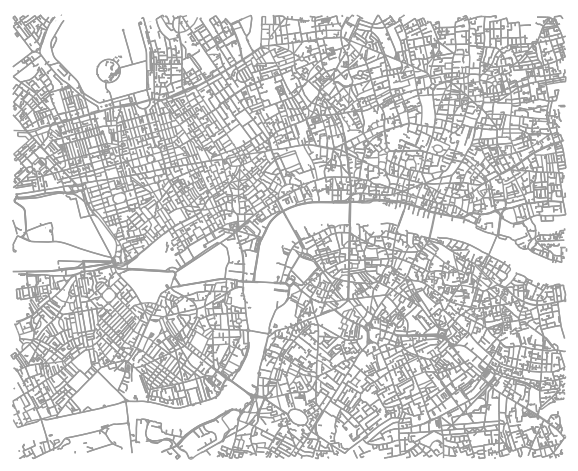
\includegraphics[width=1\linewidth]{bbox_bike_1_filter_cropped}
  \caption{1: most confident cyclists}
  \label{fig:sub1}
\end{subfigure}%
\begin{subfigure}{.5\textwidth}
  \centering
  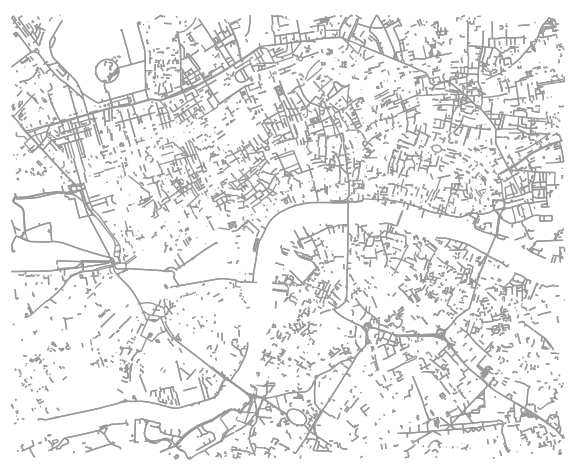
\includegraphics[width=1\linewidth]{bbox_bike_5_filter_cropped}
  \caption{5: no interaction with cars }
  \label{fig:sub2}
\end{subfigure}
\caption{Edges included by different filters}
\label{fig:test}
\end{figure}

\begin{figure}
\centering
\begin{subfigure}{.5\textwidth}
  \centering
  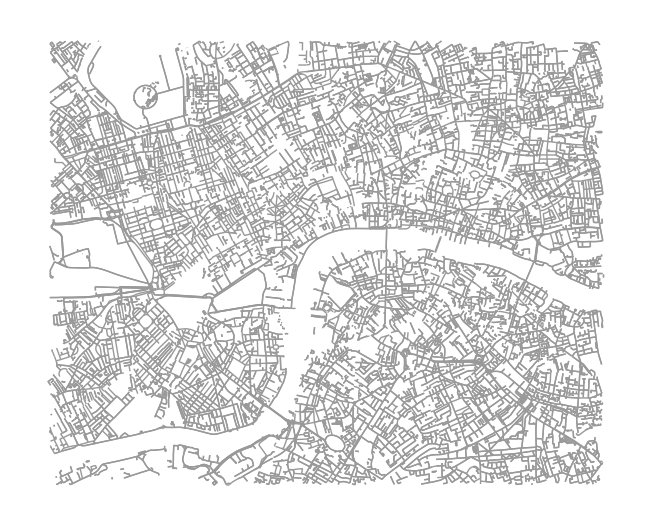
\includegraphics[width=1\linewidth]{bbox_bike_2_filter_cropped}
  \caption{2: all but primary streets}
  \label{fig:sub1}
\end{subfigure}%
\begin{subfigure}{.5\textwidth}
  \centering
  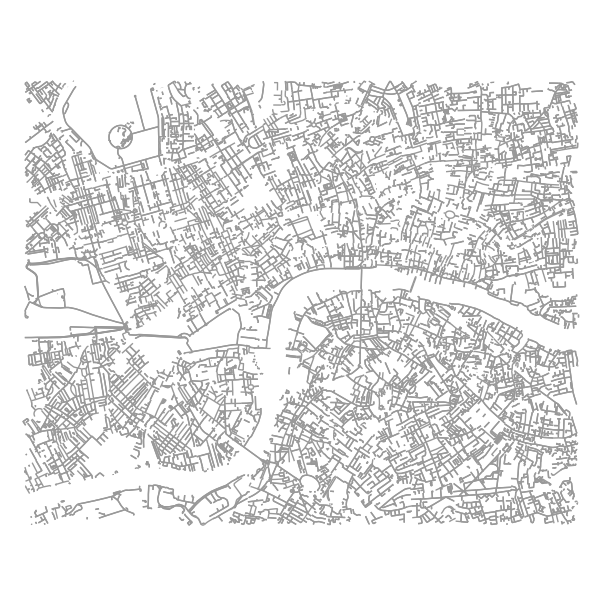
\includegraphics[width=1\linewidth]{bbox_bike_4_filter_cropped}
  \caption{4: only residential and living streets}
  \label{fig:sub2}
\end{subfigure}
\caption{Edges included by different filters}
\label{fig:test}
\end{figure}


%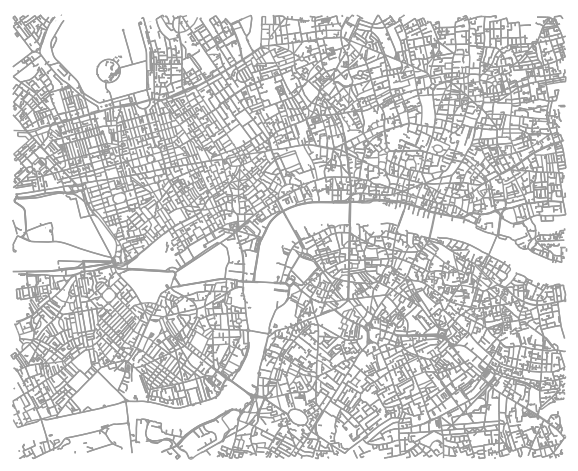
\includegraphics{bbox_bike_1_filter_cropped}

%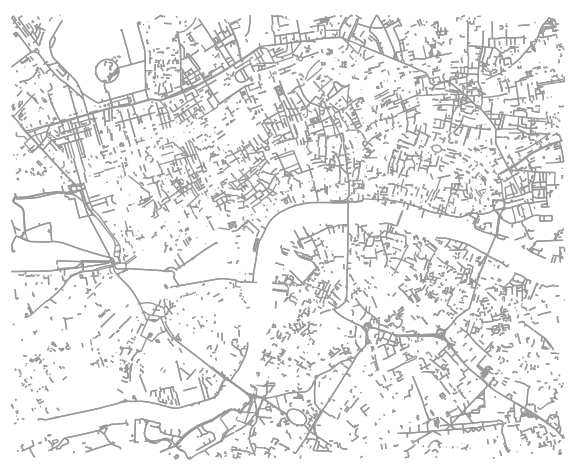
\includegraphics{bbox_bike_5_filter_cropped}
Level\_1

no interaction with cars

Level\_2

level\_1 plus living streets and residential streets

Level\_3

all streets 

Undirected

Theoretical Cycle Network

\subsection{Network Characteristics}



chart of largest connected component of network as edge types are included. 

no cars,
+ living streets
+ residential streets
+ tertiary 
+ secondary
+primary

\subsection{Travel Times}

\subsection{test for differences}

\subsection{Cycling Danger}

\subsection{Accessibility}

%%%%%%%%%%%%%%%%%%%%%%%%%%%%%%%%%%%%%%%%%%%%%%%%%%%%%%%%%%%%%%%%%%%%%%%%%%%%%%%%%%%%%%%%%%%%%%%%%%%%%%%%%%%%%%%%%
\section{Conclusions}

\subsection{Results}

\subsection{Limitations}

\subsection{Opportunities for improvement and extension}




%%%%%%%%%%%%%%%%%%%%%%%%%%%%%%%%%%%%%%%%%%%%%%%%%%%%%%%%%%%%%%%%%%%%%%%%%%%%%%%%%%%%%%%%%%%%%%%%%%%%%%%%%%%%%%%%%
\section{Appendix}




\begin{itemize}
\item one
\item two
  \begin{itemize}
  \item one point one
  \item one point two
  \end{itemize}
\end{itemize}

\subsection{Subsection 1}

\begin{figure}
\centering
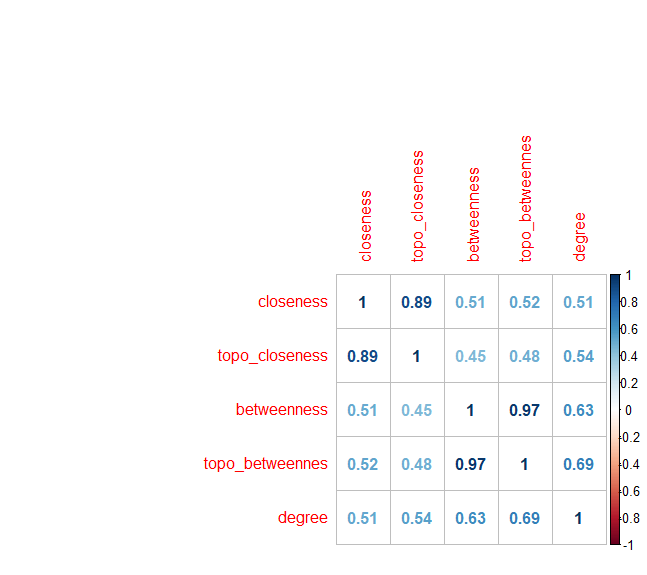
\includegraphics[width=0.8\textwidth]{example}
\caption{Correlation between station/node metrics}
\end{figure}





\begin{tabular}{lrl}
tag & count & definition \\
bridleway& 46 & For horse riders\\
crossing & 2 & A crosswalk \\
cycleway & 4726 & Designated Cycleway\\
living street & 153 & Pedestrians have legal priority over cars. Low speeds.\\
no & 2 & Not an official tag \\
path & 2432 & Generic, including footpaths, cycle paths, bridleways and tracks. \\
pedestrian & 1650 & Roads mainly/exclusively for pedestrians.\\
permissive & 2 & Not an official tag\\
primary & 6668 & Important roads linking larger towns.\\
primary link & 97 & link roads associated with primary roads.\\
residential & 30021 & Roads that serve access to housing, without connecting settlements.\\
 road & 4 & A highway of unknown type. \\
secondary & 3272 & Less important than primary.\\
secondary link & 46 & link roads associated with secondary roads.\\
service & 16474 & Access roads to industrial or business parks, etc. \\
tertiary & 5602 & Less important than secondary\\
tertiary link & 26 & Link roads associated with tertiary roads. \\ 
track & 492 & Roads for mostly agricultural or forestry uses. \\
trunk & 2683 & Important roads that aren't motorways. \\
trunk link & 134 & Link roads associated with trunk roads \\
unclassified & 7637 & less important than tertiary. Artefact of UK road system.\\ 
\end{tabular}




\begin{tabular}{|l|l|l|l|}\hline
  \multirow{10}{*}{numeric literals} 				& \multirow{5}{*}{integers} 	& in decimal 					& \verb|8743| \\ \cline{3-4}
  					    				& 				       	& \multirow{2}{*}{in octal}   		& \verb|0o7464| \\ \cline{4-4}
  					    				& 					& 						& \verb|0O103| \\ \cline{3-4}
  					    				& 					& \multirow{2}{*}{in hexadecimal}	& \verb|0x5A0FF| \\ \cline{4-4}
 				 	    				& 					& 						& \verb|0xE0F2| \\ \cline{2-4}
  					    				& \multirow{5}{*}{fractionals} 	& \multirow{5}{*}{in decimal} 		& \verb|140.58| \\ \cline{4-4}
 				 					& 					& 						& \verb|8.04e7| \\ \cline{4-4}
  									& 					& 						& \verb|0.347E+12| \\ \cline{4-4}
  									& 					& 						& \verb|5.47E-12| \\ \cline{4-4}
  									& 					& 						& \verb|47e22| \\ \cline{1-4}
  \multicolumn{3}{|l|}{\multirow{3}{*}{char literals}} 													& \verb|'H'| \\ \cline{4-4}
  \multicolumn{3}{|l|}{} 																	& \verb|'\n'| \\ \cline{4-4}          %% here
  \multicolumn{3}{|l|}{} 																	& \verb|'\x65'| \\ \cline{1-4}        %% here
  \multicolumn{3}{|l|}{\multirow{2}{*}{string literals}} 												& \verb|"bom dia"| \\ \cline{4-4}
  \multicolumn{3}{|l|}{} 																	& \verb|"ouro preto\nmg"| \\ \cline{1-4}          %% here
\end{tabular}




\begin{verbatim}
use pseudocode
\end{verbatim}

\textit{italics}
\textbf{bold}

XXXX words excluding headings, figures, and references. \\

%\nocite{*}
%
%\medskip
%
%
%\printbibliography




%%%%%%%%%%%%%%%%%%%%%%%%%%%%%%%%%%%%%%%%%%%%%%%%%%%%%%%%%%%%%%%%%%%%%%%%%%%%%%%%%%%%%%%%%%%%%%%%%%%%%%%%

%%%%%%%%%%%%%%%%%%%%%%%%%%%%%%%%%%%%%%%%%%%%%%%%%%%%%%%%%%%%%%%%%%%%%%%%%%%%%%%%%%%%%%%%%%%%%%%%%%%%%%%%

%%%%%%%%%%%%%%%%%%%%%%%%%%%%%%%%%%%%%%%%%%%%%%%%%%%%%%%%%%%%%%%%%%%%%%%%%%%%%%%%%%%%%%%%%%%%%%%%%%%%%%%%

%%%%%%%%%%%%%%%%%%%%%%%%%%%%%%%%%%%%%%%%%%%%%%%%%%%%%%%%%%%%%%%%%%%%%%%%%%%%%%%%%%%%%%%%%%%%%%%%%%%%%%%%

start of lit review

\section{Introduction}

More than half of the world's population lives in cities. Cycling is of obvious importance to the well being of the world's  urban population in terms of the macro-climate crisis, local pollution problems, and public health issues. A commonly researched question is ``what factors have the most significant effect on cycling rates?''

This literature review will show that existing research is limited by two considerations. First is the scope of the analysis, considering individual changes instead of the status of the entire transportation network from the cyclists perspective.  Second is the difficulty of obtaining data used by the studies that do take a comprehensive network approach. 

After critically reviewing this existing research, a methodology for using open source tools and data to estimate the relative strength of a cycle network and a method for prioritizing improvements will be specified. 

\section{Discrete Approach}

\section{Network Approach}

\section{Intended Methodology}







\section{Basic Framework}

The goal of this research is to assess the quality of the London Cycle Network. How well does it serve its users? To do this, first I'll review traditional literature on the impact of infrastructure improvements on the rate of cycling, which will make it clear that only a comprehensive view of cycling infrastructure, analysis of the full network, can allow an accurate understanding. The limited work available that applies network analysis to cycling infrastructure will be reviewed. Before specifying research questions and methodologies, general network analysis literature relevant to this work will be reviewed. 


\section{Introduction}

More than half of the world's population lives in cities. Cycling is of obvious importance to the well being of the world's  urban population in terms of the macro-climate crisis, local pollution problems, and public health issues. A commonly researched question is ``what factors have the most significant effect on cycling rates?'' The review of literature that follows will argue that the majority of work on this question approaches the matter from a perspective of discrete policy intervention and the effect of marginal improvements on cycling. This fails to build a comprehensive theory of cycling rates that a network analysis approach can offer. Only network theory can offer a high level look at the level of service in a community. The review that follows takes the structure of an initial look at typical literature considering how to promote cycling, recent attempts to use network analysis to accomplish this same goal, and closes with a look at work in network analysis that can inform applying the field to cycle networks. The overarching theme of the review and the research that is proposed is the idea that no individual intervention is sufficient to change behavior until a comprehensive network of infrastructure that reflects the importance of locations according to centrality is created. The implication of this view is that infrastructure changes are unlikely to have a meaningful effect on behavior in the system until a critical mass or tipping point is reached in the network. 

Basic attitude is that improvements to infrastructure only matter to the extent that they improve safe connectivity to ``important'' nodes/edges. 

%%%%%%%%%%%%%%%%%%%%%%%%%%%%%%%%%%%%%%%%%%%%%%%%%%%%%%%%%%%%%%%%%%%%%%%%%%%%%%%%%%%%%%%%%%%%%%%%%%%%%%%%%%%%%%%%%%

\section{Literature Review}

\subsection{Relevant Literature regarding cycling generally}

The most important conclusions from literature that tries to predict cycling behavior is the focus on multiple types of cyclists, and the factors that influence each type's decision to cycle. Most often, four types of cyclists are used, ``strong and fearless'', ``enthused and confident'', ``interested but concerned'', and ``no way no how'' (\cite{dill2013four}). This categorization is sometimes changed to follow demographics, focusing on young, generally male, adults, older adults, and childern. CITE. The literature separates the decision to cycle into the decision of cycling frequency, how often someone who is willing to cycle generally chooses to do so, and the decision to cycle at all, with different factors influencing each decision (\cite{stinson2005comparison}). 

Despite behaviorial differences between these categories, research has shown that all cyclists are willing to sacrifice time and energy for increased safety on their route. CITE. Indeed, psychological research showed that fear is a significant factor during an urban cycling trip (\cite{ellett2018state}). This is important given the sensitivity cyclists show to efficiency. CITE. The impact of a route change can be very significant, for instance a higher frequency of stop signs on a route can double the energy required for a journey (\cite{fajans2001bicyclists}). Given the common trade off between efficiency and safety, it was found that the effect of infrastructure improvements is very dependent on context, effect is a function of the change in safety, and the importance of the location to trips (\cite{kondo2018bike}), improvements that meaningfully increase safety at important locations have the largest effect. 

Several studies looked at the importance of perception in behavior change, assuming that a real change in safety is irrelevant if it is not perceived by potential cyclists as a change(\cite{li2012physical} and \cite{parkin2007models}). This gives rise to literature that focuses on a behavior and attitude change approach from psychology the prioritizes change in habits and perception over infrastructure, with changes to the built environment only used where required to change perception (\cite{savan2017integrated}). This should be considered in the context of research showing that cyclist perceptions of danger are generally accurate (\cite{vandenbulcke2014predicting}). Thus it seems reasonable to conclude that despite the decision to cycle being a fairly complex mix of factors, the decision for almost any urban commuter, comes down to safety, and efficiency. An efficient network of safe edges, connecting important nodes, would be expected to have a meaningful effect on the rate of cycling in an urban area.  

%Gosse, Estimating Spatially and Temporally continuous bicycle volumes by using sparse data. Difficult to get an estimate of bike traffic with the data available. \cite{gosse2014estimating}
%
%Gu, The cost effectiveness of bike lanes in New York City, ROI is high for bike lanes. \cite{gu2017cost}
%
%Heinen, Commuting by bicycle, an overview of the lit: investigates the determinants for commuting by bicycle. \cite{heinen2010commuting}
%
%Kondo: Where do bike lanes work best a Bayesian spatial model of bicycle lanes and bicycle crashes. Bike lanes have different values in different places. \cite{kondo2018bike}
%
%Li, Physical environments influencing bicyclists' perception of comfort on separated and on-street bicycle facilities. Simple look at perceived safety in different cycling environments. \cite{li2012physical}
%
%Parkin, Models of perceived cycling risk and route acceptability. The factors that influence perceived safety \cite{parkin2007models}
%
%Savan, Integrated Strategies to accelerate the adoption of cycling for transportation, Psychological behavioral change approach to increasing cycling. \cite{savan2017integrated}
%
%Stinson, Route preferences of experienced and inexperienced bicycle commuters. Different types of cyclists react differently to traffic stress. \cite{stinson2005comparison}
%
%Thigpen, States of change approach to explore opportunities for increased bicycle commuting. Focuses on changing cyclists rather than infrastructure. \cite{thigpen2015using}
%
%Vandenbulcke, Predicting cycling accident risk in Brussels: A Spatial case control approach. The things cyclists perceive as dangerous are dangerous. \cite{vandenbulcke2014predicting}

%%%%%%%%%%%%%%%%%%%%%%%%%%%%%%%%%%%%%%%%%%%%%%%%%%%%%%%%%%%%%%%%%%%%%%%%%%%%%%%%%%%%%%%%%%%%%%%%%%%%%%%%%%%%%%%

\subsection{Literature addressing cycling From a network perspective}


\cite{buehler2016bikeway} is a very useful introduction to the literature on cycling networks. Unfortunately it concludes that very little true network analysis has been developed for cycle networks. The majority of papers they found could be categorized into those that focus exclusively on nodes, and those that focus on edges of the dual graph, where intersections are nodes and streets are edges. At the time of writing there were 115 papers citing Buehler's review, however all but 5 of them fail to take Buehler's central recommendation that \textit{If individual characteristics of a network's links and nodes contribute to cycling levels, it logically follows that a network of such features would as well...}. The ``Toward Studying the Whole Bicycling Network'' section of Buehler's review is a good overview of attempts up to 2016. The key findings were that continuity and connectivity of infrastructure is valued by cyclists. Of particular interest is the \cite{schoner2014missing} study of the relationship between network characteristics and cycling mode share in 74 US cities. That study found density of the network had the highest elasticity for effect on cycling rate. 

Several of the works reviewed contribute new ways of measuring ``quality'' of the infrastructure, these quality measures include a Bicycle Compatibility Index (BCI) (\cite{klobucar2007network}),  Bicycle Level of Service (BLOS) (\cite{lowry2012assessment}), and Level of Traffic Stress (LTS) (\cite{mekuria2012low}). Each of these can reasonably be viewed as an attempt to measure the ``safety'' of a network link. These studies generally lacked a rigorous method for prioritizing nodes by importance or defining a sample set of trips between nodes. Improvements to this will be addressed in the section reviewing network analysis literature. 

Buehler notes that a key challenge to using the network methods reviewed is data availability, this research hopes that network analysis can be a method for reducing rather than extending the amount of data necessary to understand a cycle network, as network statistics could be used to replace some empirical measurements as discussed below.  They further criticize the approaches as lacking empirical validation. Gathering accurate cycle traffic data and safety data is an immense challenge as demonstrated by the flow estimation techniques of \cite{gosse2014estimating} and the safety estimate techniques of \cite{puchades2018role}, which focuses on near misses as a proxy for predicting actual safety incidents, but acknowledges the difficulty of collecting near miss data without human observation. CITE. 

Since the publication of Buehler's review, the papers extending the full network analysis method have had moderate success. \cite{akbarzadeh2018designing} uses taxi trip data to weight the links between destinations in order to build communities of nodes that tend to be origin and destination pairs. While this is a novel approach to prioritizing edges, taxi usage tends to be for less frequent travel between nodes and the general literature as well as this work focuses on daily commuting, which is rarely accomplished by taxi. \cite{boisjoly2019bicycle} focuses on the directness of routes on cycle paths between nodes. 

\cite{doorley2019designing} focus on building cycle infrastructure to maximize a function of travel costs, infrastructure costs, health, traffic accidents, and pollution. While this is an interesting approach, it addresses a more political question in the sense that the key result of the algorithm is to recommend a specific amount of investment in cycle infrastructure to maximize the costs and benefits to all road users, The author's fail to recognize the prioritizing the goals of public policy is a highly normative and subjective exercise and that a model designed to give an ``objective'' answer to this question inherently reflects the author's preferences and when calibrated to ``the real world'' reflects the biases and preferences of the status quo, rather than the true ideal outcomes preferred by a population. Instead, modeling, especially for urban planning purposes, should accept an exogenous goal and implement it as efficiently as possible. For instance, cycle infrastructure, is explicitly intended to reduce motor vehicle use, it would make no sense to then use a model that determines the efficient level of motor vehicle use, the political process has already determined the answer and merely asks for implementation recommendations from the modeler. 

\cite{mauttone2017bicycle} similarly focuses on an optimization framework for cycling networks, choosing a subset of streets that are ``suitable to building cycle infrastructure''. This is odd in the sense that the goal of building cycle infrastructure is to \textit{create} streets that are suitable for cycling, not merely identify them. Similar to \cite{doorley2019designing}, they identify a cost to building cycle paths which they seek to balance against the benefits. 

Overall, it is not clear that a model for building cycle paths should be particularly cost sensitive. \cite{gu2017cost} found a very high return on investment to the budget for cycling infrastructure in New York City. The very idea of using network analysis for the development of cycle networks emphasizes the potential non linearity of the effect of building more infrastructure, with usage accelerating as the network approaches ``completeness'' in some for. In addition, cities tend to combine cycle infrastructure improvement with other required improvement and maintenance activities, mitigating the costs by being opportunistic in implementation. 

Lastly, \cite{osama2017models} uses a number of predictors including network statistics to predict bike travel within zones of Vancouver similar to \cite{schoner2014missing}. They found a positive coefficient for the density of the bike network in the zone. 

Thus while network analysis has been applied to cycle infrastructure, clearly there is not a consensus on the methodology. In particular, a definition of ``quality'' or ``safety'' has not been established. Additionally, a method for exploring the network of infrastructure defined is still lacking. Lastly,  

%5 papers since Buehler:
%\begin{itemize}
%
%\item \cite{boisjoly2019bicycle}
%\item \cite{akbarzadeh2018designing}
%\item \cite{doorley2019designing}
%\item \cite{mauttone2017bicycle}
%\item \cite{osama2017models}
%
%\end{itemize}




%%%%%%%%%%%%%%%%%%%%%%%%%%%%%%%%%%%%%%%%%%%%%%%%%%%%%%%%%%%%%%%%%%%%%%%%%%%%%%%%%%%%%%%%%%%%%%%%%%%%%%%%%
%
%
%Akbarzadeh, Designing Bike networks using the concept of network clusters, Taxi trips to indicate links between nodes. Not a very good method for understanding where to build networks, needlessly complicated. \cite{akbarzadeh2018designing}
%
%
%Data from online survey to get a cost function, predicted travel routes, compared to shortest route, which is used to measure network connectivity. 
%%%%%%%%%%%%%%%%%%%%%%
%
%\textbf{
%Counter intuitively, if one was to measure the total distance of the network, that would be an incentive to build less direct links, since these tend to be longer.}  
%%%%%%%%%%%%%%%%%%%%%%%
%\cite{boisjoly2019bicycle} 
%
%Buehler \& Dill's  particularly helpful review of literature on bike networks uses a framework that groups the literature by two categories, that focusing on the links of the network, different types of cycle lanes, and that focusing on the nodes of the network, intersections. It ends by addressing the possibility of a cohesive study of a bicycle network holistically.
%
%	For instance \textit{One study linked cycling levels to self reported measures of the bicycling environment, including being able to take shortcuts on a bicycle compared to routes available to cars. This measure of connectivity was found to be significant (Titze, Stronegger, Janschitz, \& Oja, 2008).}
%	
%	\textit{ a recent paper using aggregate bicycle commuting data from 74 US cities (Schoner \& Levinson, 2014). The authors develop several different measures that represent the size, connectivity, density, fragmentation, and directness of the bicycle network. The density of the bikeway network (all types of facilities combined) had the largest elasticity value, larger than connectivity, fragmentation, and directness combined.}
%	
%	This includes a Bicycle Compatibility Index (BCI) combination of distance and safety, Bicycle level of service (BLOS) from ``Highway Capacity Manual'', \cite{Lowry} and Level of Traffic Stress (LTS) \cite{Mekuria and Furth} a four point scale based on architectural features of the route.
%	
%	Basically, these four don't really constitute a holistic approach still. 
%	
%	Difficulty of validating the effect because there isn't a lot of cyclist behavior data available.
%	
%	
%Since Buehler's literature review was published 115 subsequent papers have cited it but only a few have taken the author's central recommendation that a holistic approach to evaluating a bike network be employed. 
%
%
%Starting point for the lit review since it covers everything prior to 2016, node, link and network focused lit. 
%\cite{buehler2016bikeway}
%
%Edmonton did a rapid full network implementation instead of a incremental approach. 
%\cite{cabral2019low}
%
%Genetic algorithm used to solve a mathematical program with equillibrium constraints. 
%\cite{doorley2019designing}
%
%Optimization problem: retrofitting existing roadway infrastructure for bicycles. Minimize cost while conncting all origin destination pairs considering bicycling level of service. 
%\cite{duthie2014optimization}
%
%San Jose, vizualizing and analyzing lack of connectivity. 
%First low stress network analysis. Focuses on \% of pairs connected with low stress links. A few improvements would dramatically increase connectivity. 
%\cite{furth2016network}
%
%Seattle , tool for analyzing low stress connectivity. 
%\cite{lowry2016prioritizing}
%
%Compare connectivity for different types of cyclists in different neighborhoods. 
%\cite{lowry2017quantifying}
%
%Algorithm for bicycle network design: balance interests of users and planners, construction v user cost, proportional to distance, adjusted for usage rates, and ``discontinuities'' 
%\cite{mauttone2017bicycle}
%
%Original study on low stress network connectivity
%\cite{mekuria2012low}
%
%%\cite{macmillan2017understanding}
%
%Algo for bike network design, filter out ``ineligible streets'' then balance between improvement for cyclists and cost for drivers, then optimize with genetic algorithm, 
%\cite{mesbah2012bilevel}
%
%%\cite{milakis2012planning}
%
%Predicting bike kilometers traveled with network indicators, land use and road facility. Vancouver Canada. Bayesian model with spatial random effects. 
%\cite{osama2017models}
%
%Schoner's study was a regression of cycling mode share on the network characteristics of 74 US cities. This is the closest study to what I'm intending to do for London. Basically apply the results of that study to London. 
%\cite{schoner2014missing}
%
%
%Does level of traffic stress explain bicycle travel behavior. Uses census data , mode choice data, and regional household survey data to test relationship between traffic stress and bicycle travel behavior. Questions LTS. 
%\cite{wang2016does}


%%%%%%%%%%%%%%%%%%%%%%%%%%%%%%%%%%%%%%%%%%%%%%%%%%%%%%%%%%%%%%%%%%%%%%%%%%%%%%%%%%%%%%%%%%%%%%%%%%%%%%%%%%%%%%%%%%


\subsection{Network analysis Literature relevant to the research methodology proposed}

\textit{note: this section should probably be worked into the review of cycle network analysis above instead of separated out. Combine criticisms of existing work and solutions from network science.}

This work intends to improve upon the work detailed above through the inclusion of more ideas from network science that can improve and extend and simplify the models already specified. 

There are a number of considerations from network analysis literature that can complement the work already applying the field to cycling networks. Perhaps the most important is the idea that the transportation network and the location of activities in a city reinforce each other. The most productive activities that occur in a city tend to be the most easily accessed according to central place theory. This has been shown empirically for instance by \cite{porta2012street} and by \cite{wang2011street}. In the literature discussed above authors address the key change in networks of defining a computationally feasible set of trips between nodes in a few different ways. This is misguided though as network theory offers a number of tools for exploring a graph efficiently. A random walk weighted by a centrality measure will tend toward trips between more important nodes because these tend to be more central. For instance \cite{Jiang2009characterizing} or  \cite{volchenkov2007random} both show that weighted random walks can do a accurate job of representing human activity on a street network. 

A number of network statistics are used in the literature reviewed above. \cite{crucitti2006centrality} complements these as the centrality and connectedness measures used should be more formally justified according to network theory. 

While, the multiplex offers an interesting approach to studying the interaction between bicycle usage and train and bus, this is beyond the scope of this work and perhaps beyond the scope of London , where bicycles are not generally allowed on public transport, unlike some other cities. 

The potential for a ``transition'' in the cycle network per \cite{barthelemy2018transitions} is an exciting possibility. Finding edges that need to be added to a network in order for a transition in network connectivity to occur is a valuable exercise. In addition, specifying network characteristics according to those specified by \cite{barthelemy2011spatial} is also very valuable. 

Overall there are a number of considerations from network science that this research intends to add to the analysis of cycle networks. The exact implementation of these considerations will be specified in the methodology section. 

%\textbf{
%The key questions that need to be addressed by this lit are: 
%\begin{itemize}
%\item How to rigorously compare distributions of centrality?
%\item Dual or Primal graph? 
%\item How to actually do what I intend to do, a manual of some sort?
%\item Anything to do with growing one network on top of another. 
%\item Address and dismiss multiplex  networks approach.
%\item The potential for a ``transition'' in the network?
%\item Which centrality indices to use?
%\item Justify centrality as a way of prioritizing connectivity as a shortcut.  i.e. use centrality to weight nodes. 
%\item Community identification in planar graphs? 
%\item Could a weighted random walk be a good proxy for trips? 
%\item Could it make sense using the dual graph, to add an edge to ach intersection node so that the node could be a destination but also include information about the level of stress associated with traveling through the node? 
%\end{itemize}
%}
%
%Crossover from scale free to spatial network:
%
%What is distinct about spatial networks: distance weighted, preferential attachment and distance selection. When distance effect is significant, connectivity dist has a cutoff depending on node density, clustering coeff is very high, assortivity, positive max to degree correlation
%\cite{barthelemy2003crossover}
%
%Spatial Networks:
%
%relevant part is the review of processes that take place on spatial networks. 
%Phase transitions, random walks, synchronization, navigation, resilience, disease spread. 
%\cite{barthelemy2011spatial}
%
%Probably the most interesting because using percolation, as edges are added to a spatial network, a ``giant component'' suddenly emerges that connects the majority of nodes. This could be the specific goal of the research, how close is the London cycle network to this type of transition? 
%\cite{barthelemy2018transitions}
%
%Centrality Measures in spatial networks of urban streets. Uses 4 indices of centrality: closeness, betweenness, straightness, information. 
%\cite{crucitti2006centrality}
%
%Nonparametric resampling of random walks for spectral network clustering.
%goal is to assess the statistical significance of clustering and robustness of community identification. 
%\cite{fallani2014nonparametric}
%
%5 proxies for resilience in the urban form: diversity, redundancy, modularity, connectivity, efficiency. 
%Scales: plot, street, block, district.
%\cite{feliciotti2016design}
%
%
%Correlations in Multiplex networks. Competing v complementing layers of multiplex networks have positive or negative correlations. \cite{nicosia2015measuring}
%
%These two can inform the choice between primal and dual graphs for this project. Different measures of accessibility and their normative consequences. \cite{paez2012measuring}
%
%Multiple Centrality assessment for streets as nodes. 
%\cite{porta2006primal}
%
%Intersections are nodes, streets are edges
%\cite{porta2006dual}
%
%Street Centrality and the location of economic activities in Barcelona. Very useful because many previous studies used a subset of locations as ``important nodes'' but I could just prioritize by centrality since that is related to the importance of a destination. 
%\cite{porta2012street}
%
%
%Street centrality and land use intensity in baton rouge. Same as Porta 2012, more central streets have more going on. People tend to spend more time on more central streets. 
%\cite{wang2011street}
%
%Planar graphs
%Connection between centrality and economic activity
%	Porta 2012, Barcelona
%Transitions in spatial networks: percolation and small world stuff
%Multiplex networks probably not relevant because it's hard to take a bike on a train or bus or whatever
%	Urban accessibility measurement: Porta , Biazzo, Need to weight edges but inverse of distance.

%%%%%%%%%%%%%%%%%%%%%%%%%%%%%%%%%%%%%%%%%%%%%%%%%%%%%%%%%%%%%%%%%%%%%%%%%%%%%%%%%%%%%%%%%%%%%%%%%%%%%%%%%%%%%%%%%%

\section{Most optimistic Project Plan/Methodology}

Goal is to quantify the quality of the London Cycling Network with the working assumption that a better network has a meaningful positive effect on the rate of cycling in a city. 

The first step in this investigation is to build a data set that represents the London cycling network as accurately as possible. This representation needs to reflect the fact that different cyclists are willing to use different streets as a function of the perceived safety of the street and the level of confidence of that cyclist. Thus the data set will be multiple representations of the city cycling network that each represent a level of confidence, only including streets with a certain level of safety. 

A key question then is, how to quantify ``safety''. In a perfect world, this would be done empirically. This would involve a combination of cycle traffic volume collection, cycle traffic behavior observation, and interviews with a representative set of cyclists and non-cyclists about their decision making. All of this data could be compared to the cycling environment in different locations to find cyclist sensitivity to different factors.  

The literature provides a number of methods, which will be explored to the fullest extent possible. Factors that will be considered include, the presence of dedicated bike infrastructure, traffic volumes, traffic speeds, road characteristics, historical traffic incidents, and intersection characteristics. 

Once the network has been quantified in this way, two basic methods will be applied to evaluate it. The first is to compare the distribution of edges by centrality for each of the networks. Are cars and high confidence cyclists at a significant advantage in terms of the edges available to them compared to lower confidence cyclists? Does does the centrality of edges allowed under the most conservative standards explain many Londoner's choice not to cycle at all? 

The second method is intended to extend the first. Looking at the distribution of centrality is unable to reveal the network's actual service for common trips between important nodes on the network, because a high number of very central but disconnected edges is not as useful as a high number of high centrality edges with high connectivity. To investigate this, a random walk between nodes, weighted by node importance will be used. This will build a sample of trips and statistics about the random walk can be used to compare the experience of representative users of different networks. 

Finally, the possibility of a ``transition'' in the networks defined will be explored. What changes to the network are required for a dramatic change in connectivity to occur? This is the most uncertain but potentially most valuable part of the research. Past research has analyzed the linear individual effect of cycling infrastructure, but has not considered the possibility of a rapid acceleration in cycling usage as the result of a network wide transition in connectivity. 

Finally, community identification could be applied to the networks to find whether particular neighborhoods in London are especially good for cyclists. 


\section{Data considerations}

I still need to spend a lot of time with OSM, networkx, and the London data store. 

OSM has street network data, bike network data and some road characteristics. 

Networkx should be able to turn this data into a usable file. 

The London data store has traffic incident data but I haven't found data with exact locations yet

There is traffic volume data but it's at a few thousand observation points, so a continuous data set needs to be estimated. 

I think OSM is my only source for street characteristics, not clear that it's accurate or up to date.


Official data for cycle infrastructure is from 2014: \href{https://data.gov.uk/dataset/47f0a282-3356-4530-8e7b-f67aaf4bec63/cycle-routes}{link}

This says it's updated and maybe integrated into OSM? \href{https://www.cyclestreets.net/blog/category/open-data/}{link}

Press release about data set \href{https://www.london.gov.uk/press-releases/mayoral/action-plan-to-get-more-londoners-cycling}{link}

But no actual data. Seems like OSM is the delivery mechanism, unclear how integrated the data is into OSM. 


\section{Going Forward}


\subsection{Questions}

Data status, it seems like the basic data required for the work exists but it isn't clear how to access it and how to match different data sets up with each other. 

Methodology status, clearly the methodologies I intend to use are possible, they're used in other papers, but I need to find manuals/text books that actually discuss how to implement the methods. 

\subsection{Tasks}

\subsubsection{Data}
		\begin{itemize}
			\item Geoff Boeoing network X OSM tutorial
			\item read through Talk GB mailing list for OSM info
		\end{itemize}

\subsubsection{Analysis}
		\begin{itemize}
			\item centrality distribution comparison method
			\item weighted random walk method
			\item ``transition'' identification method
			\item ``community detection method
		\end{itemize}


%%%%%%%%%%%%%%%%%%%%%%%%%%%%%%%%%%%%%%%%%%%%%%%%%%%%%%%%%%%%%%%%%%%%%%%%%%%%%%%%%%%%%%%%%%%%%%%%%%%%%%%%%%%%%
%\section{Intended research Questions and Methodology}
%
%Overall Goal is to assess London's cycle network. 
%	Sub goal 1 is to define the London cycle network, which streets and intersections should be added to the official cycle lanes? I can use the standards from the literature cited above. 
%		Start with all nodes and edges. Delete according to standards taken from lit. 
%			standards: safety incidents, road characteristics, bike infrastructure presence, traffic data. 
%	Sub goal 2 is to define a standard to evaluate the network by. This could be, percolation, community,  detection, centrality distribution, or \% of trips possible, random walk. 
%	
%	Sub goal 3, identify the edges/nodes that are the most beneficial to add to the network. 
%	
%	Outcomes are: differences in network according to different rules. 
%	Priority of projects to add different edges/nodes to network. 
%	
%
%Possible Specific Research Questions
%	Conservative: What does London look like to a cyclist? Build network according to different rules and compare
%		traffic stress
%			intersections
%			streets
%		no right turns
%		only official bike network
%			
%			
%	Moderate: community detection using the stuff from the conservative project, where is the network the strongest? Are there parts of London with particularly good local networks? 
%	
%	
%	Aggressive: how closely has the London network followed an optimal growth of network on network? 
%		This could use standard measures of street centrality for the road network and look at accessibility for the most important streets.  
%		
%		
%		Or compare centrality distribution of bike networks to streets, use street centrality for given bike lane, are lanes relatively central or no? 
%		
%		Or compare evolution of rd networks to evolution of bike networks
%		
%Straightness is an interesting one but distance matters most I guess. 
%Congestion is not really a problem for cyclists
%
%Road network
%	attach attributes to links and nodes
%		bike lane with type
%		traffic characteristics
%		road characteristics
%		traffic incidents
%		
%Remove links and nodes according to attributes
%
%Compare distribution of centrality between estimated bike network and real road network. 
%
%Use Cycle Hire data to validate centrality preference?
%	But hires are station to station so would have to show that the probability of a station being a destination for a trip is influenced by stations centrality. 
%
%Steps:
%
%	get london road network
%		just the data
%		get the distribution of centrality measures
%	get the london bike network
%		just the data
%		get the distribution of centrality measures
%		
%	give a road an index grade
%		using accident stats and road characteristics
%		
%	add ``safe'' roads to cycle network
%	
%	compare disributions of centrality scores between road network and bike network. 
%	
%	compare network before and after Super Highway constructions
%
%%%%%%%%%%%%%%%%%%%%%%%%%%%%%%%%%%%%%%%%%%%%%%%%%%%%%%%%%%%%%%%%%%%%%%%%%%%%%%%%%%%%%%%%%%%%%%%%%%%%%%%%%%%%%

\medskip 

XXXX words excluding headings, figures, and references. \\
\pagebreak
\printbibliography


\end{document}
